\documentclass[twocolumn]{preep}

\usepackage{lipsum}

\title{A Preprint Template in \Hologo{LaTeX}}
\shorttitle{Preprint Template}

\author[1,2,3,5,*]{Paul L. Gribble}
\author[1,2,4]{Ford Prefect}

\affil[1]{ The Brain and Mind Institute, Western University, London ON, Canada N6A 3K7}
\affil[2]{ Deptartment of Psychology, Western University, London ON, Canada N6A 3K7}
\affil[3]{ Department of Physiology \& Pharmacology, Western University, London ON, Canada N6A 3K7}
\affil[4]{ Graduate Program in Neuroscience, Western University, London ON, Canada N6A 3K7}
\affil[5]{ Haskins Laboratories, New Haven CT, USA 06511}
\affil[*]{ Corresponding Author: paul@gribblelab.org}

\abstract{ Lorem ipsum dolor sit amet, consectetuer adipiscing
  elit. Ut purus elit, vestibulum ut, placerat ac, adipiscing vitae,
  felis. Curabitur dictum gravida mauris. Nam arcu libero, nonummy
  eget, consectetuer id, vulputate a, magna. Donec vehicula augue eu
  neque. Pellentesque habitant morbi tristique senectus et netus et
  malesuada fames ac turpis egestas. Mauris ut leo. Cras viverra metus
  rhoncus sem. Nulla et lectus vestibulum urna fringilla
  ultrices. Phasellus eu tellus sit amet tortor gravida
  placerat. Integer sapien est, iaculis in, pretium quis, viverra ac,
  nunc. Praesent eget sem vel leo ultrices bibendum. Aenean
  faucibus. Morbi dolor nulla, malesuada eu, pulvinar at, mollis ac,
  nulla. Curabitur auctor semper nulla. Donec varius orci eget
  risus. Duis nibh mi, congue eu, accumsan eleifend, sagittis quis,
  diam. Duis eget orci sit amet orci dignissim rutrum.  }

\keywords{human, motor learning, somatosensory cortex, force-field adaptation}


\begin{document}
\maketitle
\thispagestyle{firstpage}


\section*{Introduction}
\lipsum[2-4] Here is a citation \cite{Mattar2005-oq}. In
\cite{McGregor2016-ku} somatosensory cortex was implicated in motor
learning through visual observation.


\section*{Methods}

\subsection*{Participants}
\lipsum[6]

\subsection*{Procedure}
\lipsum[7-8]

\subsection*{Statistical Analyses}

Equation~\ref{eq:mean} shows the equation for calculating the mean of
$N$ values $X_{1}$ to $X_{N}$.

\begin{equation}
  \bar{X} = \left( \frac{1}{N}  \right) \sum_{i=1}^{N} X_{i}
  \label{eq:mean}
\end{equation}


\section*{Results}
\lipsum[9-14]

As you can see in Figure~\ref{fig:subjectmeans}, we have collected
some data already.

\begin{figure}
  \centering
  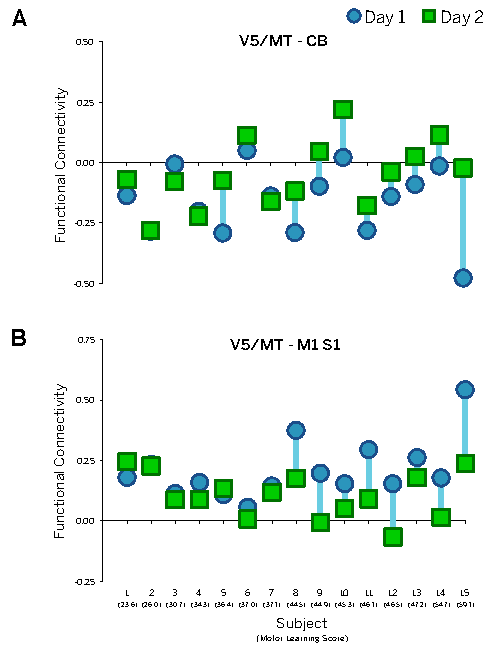
\includegraphics[width=0.95\columnwidth]{figure.pdf}
  \caption{Some data from our experiment.}
  \label{fig:subjectmeans}
\end{figure}    

Table~\ref{tab:randomjunk} shows some data organized into a table.

\begin{table}
  \centering
  \begin{tabular}{|r|l|}
    \hline
    \textbf{Value} & \textbf{Format}\\
    \hline\hline
  7C0 & hexadecimal \\
  3700 & octal \\ \cline{2-2}
  11111000000 & binary \\
  \hline
  1984 & decimal \\
  \hline
  \end{tabular}
  \caption{Some data.}
  \label{tab:randomjunk}
\end{table}

Figure~\ref{fig:percep} shows some resting-state fMRI results.

\begin{figure*}
  \centering
  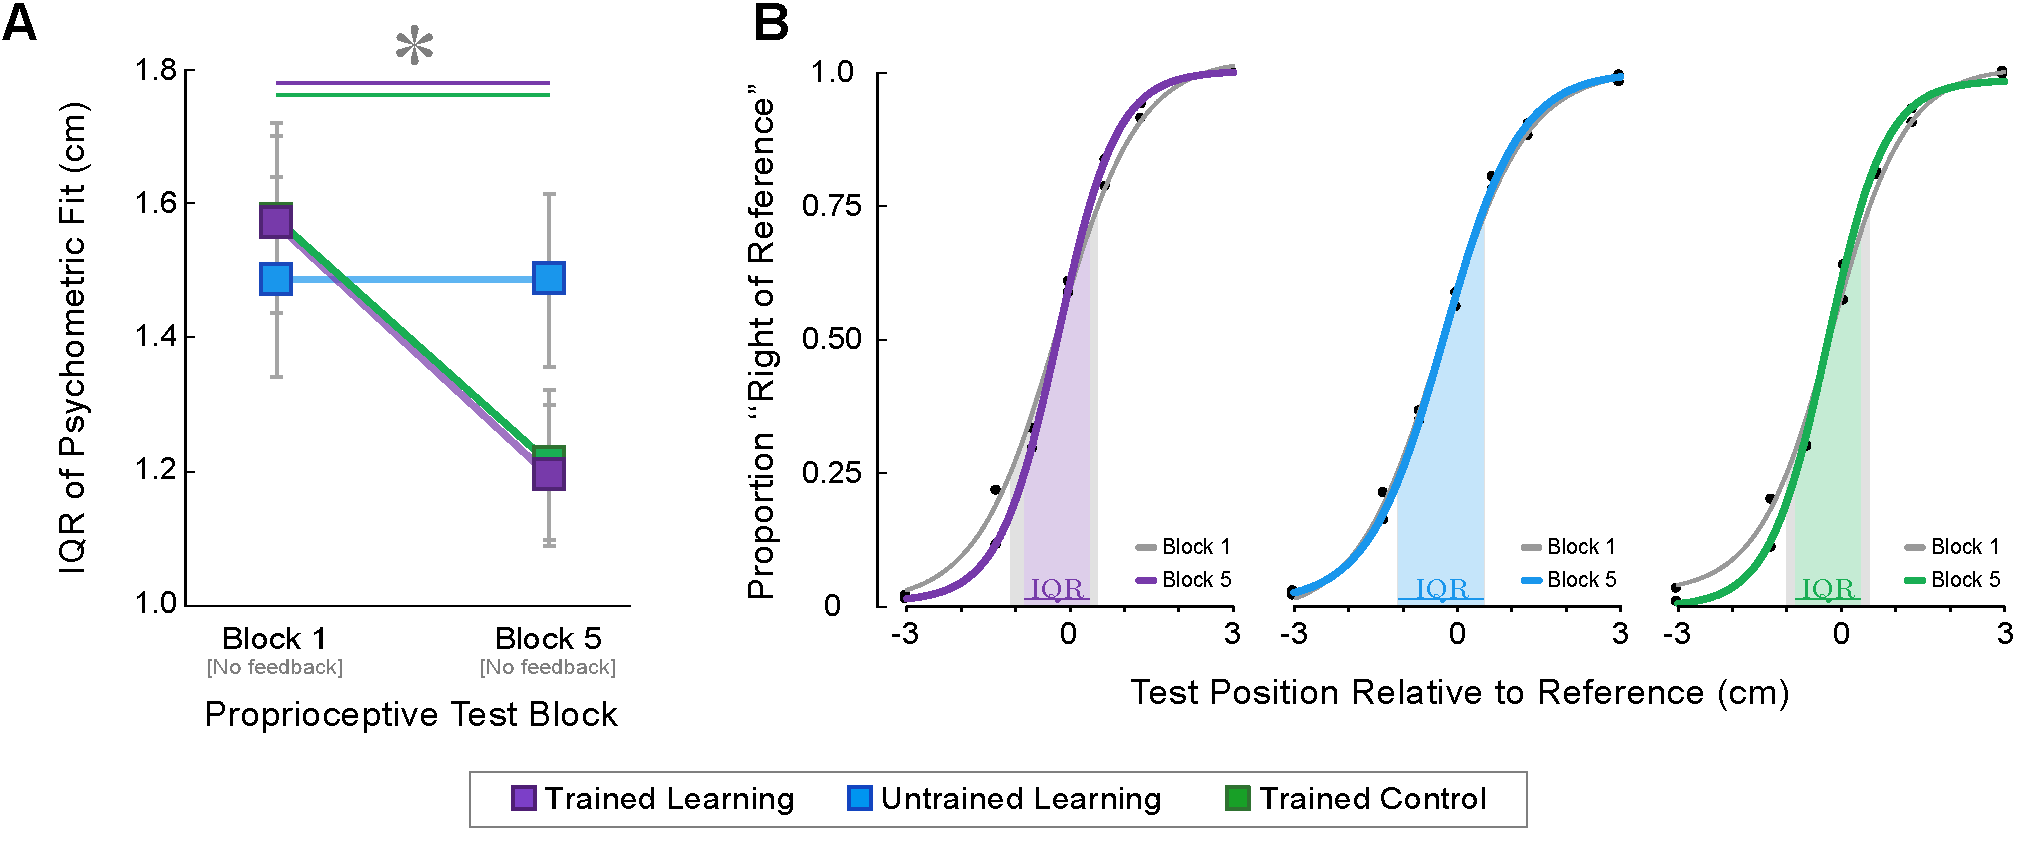
\includegraphics[width=\textwidth]{percep.pdf}
  \caption{Proprioceptive training increased proprioceptive acuity. A:
    perceptual acuity was assessed in blocks 1 and 5 of the
    proprioceptive discrimination task, during which trial-by-trial
    feedback was withheld from all subjects. Perceptual acuity was
    quantified as the interquartile range (IQR) of the psychometric
    function estimated from each subject’s set of binary responses.}
  \label{fig:percep}
\end{figure*}


\section*{Discussion}
\lipsum[15-20]


\bibliographystyle{jneurophysiol}
\bibliography{refs}


\end{document}

